\chapter{Analyse et synthèse du projet}
\label{chap:quatre}

Ce chapitre confronte les résultats obtenus aux hypothèses formulées en introduction. Il présente la solution livrée, ses performances mesurées, ses points forts et ses limites, puis les interfaces produites. Il expose enfin le coût estimatif du projet et en dresse la rétrospective.

\section{Discussion des hypothèses}
\label{sec:4-1}

Les trois hypothèses spécifiques sont reprises dans l'ordre, chacune confrontée aux mesures effectivement produites. Deux sont confirmées, une est infirmée.

\subsection{H1 --- La tenue manuelle produit une perte d'information mesurable}

\noindent\textbf{Hypothèse confirmée.}

L'hypothèse posait que la tenue manuelle du registre produit un taux mesurable de pertes d'information sur l'identité des artisans concernés et sur les valeurs élémentaires des lignes de vente. La transcription et l'analyse du registre de l'exercice~2026 la confirment sur les deux volets, et à un niveau supérieur à ce que l'observation laissait présumer.

Sur les 195~lignes de vente de la période, \textbf{41 portent un nom d'artisan que rien ne rattache au parc locatif}, soit 21,0~\%. Elles représentent 159~700~francs~CFA, c'est-à-dire \textbf{20,2~\% du chiffre d'affaires de l'exercice}. La portée de ce constat dépasse la qualité documentaire : la part artisan de ces ventes, soit environ 143~700~francs~CFA après commission, ne peut être adossée à aucun contrat d'occupation. La perte d'information a ici une contrepartie financière directe.

Ce résultat se recoupe avec la dette du village envers ses artisans. Sur le même exercice, \textbf{226~850~francs~CFA de part artisan restent à reverser}, soit 28,7~\% du chiffre d'affaires, dont 83~000~francs~CFA pour la seule Mme Justina --- laquelle porte également la plus grosse écriture non rattachable, 93~000~francs~CFA. Le bénéficiaire auquel le village doit le plus est ainsi celui dont l'identification administrative est la moins établie.

Sur le second volet, \textbf{aucune des 195~lignes ne porte les trois valeurs} quantité, prix unitaire et montant. La quantité est systématiquement absente et doit être reconstituée. Cette reconstitution est fiable lorsque deux valeurs sur trois sont présentes, mais elle signifie qu'un cinquième au moins de l'information portée par chaque ligne est produit par le traitement et non par le registre.

Deux indicateurs complémentaires précisent le tableau. 72~lignes, soit 36,9~\%, ne portent pas le corps de métier de l'artisan. Et 122~lignes seulement, soit 62,6~\%, portent une observation de décharge attestant que l'artisan a été reversé ; sur les 37,4~\% restantes, la preuve du paiement est absente du document qui devrait la porter.

Un troisième constat, non anticipé par l'hypothèse, s'est imposé à l'analyse : \textbf{l'identité du vendeur n'est enregistrée nulle part}. Une lecture antérieure avait interprété la colonne d'observation comme la portant, au motif qu'un nom de personne y figure souvent ; le rapprochement avec la feuille des commissions établit qu'il s'agit du bénéficiaire ou de l'intermédiaire d'une décharge. La perte d'information est donc plus large que l'hypothèse ne le supposait : elle porte non seulement sur le bénéficiaire de la vente, mais sur l'agent qui l'a réalisée, dont aucune trace n'existe. La règle RG-14 du système, qui enregistre l'identité de l'agent sur chaque vente, ne reprend pas une pratique existante --- elle en introduit une.

\subsection{H2 --- La centralisation produit des indicateurs jusque-là indisponibles}

\noindent\textbf{Hypothèse confirmée.}

L'hypothèse posait que la centralisation des données permet de produire automatiquement des indicateurs qui ne sont aujourd'hui disponibles qu'au prix d'un rapprochement manuel. Le tableau de bord livré la confirme : les indicateurs du la liste ci-dessus sont calculés par agrégation sur la base et actualisés à chaque consultation, là où leur établissement supposait auparavant de confronter trois supports non reliés.

Huit indicateurs sont désormais produits par agrégation et actualisés à chaque consultation : le chiffre d'affaires, les recettes de commission, le solde dû à chaque artisan, la ventilation des ventes par boutique, par artisan et par vendeur, le solde de caisse consolidé, le taux d'occupation des espaces, les produits sous le seuil d'alerte et l'état de recouvrement des redevances. Aucun n'était disponible avant ce travail autrement qu'au prix d'un rapprochement manuel entre supports non reliés, et le dernier ne l'était que sous la forme d'un relevé annuel.

L'illustration la plus nette de cette hypothèse ne porte cependant pas sur un indicateur nouveau, mais sur une question que les supports actuels ne permettent pas de trancher. La situation de caisse fait apparaître une différence de \textbf{162~525~francs~CFA} entre les avoirs dus et les sommes détenues, à côté de laquelle figurent quatre sorties datées totalisant 120~000~francs~CFA. Il est vraisemblable qu'elles expliquent l'essentiel de la différence ; rien ne permet de l'établir, faute d'un journal où ces sorties s'inscriraient dans une chronologie numérotée permettant de recalculer le solde attendu à une date donnée.

Le système répond précisément à cette configuration : le journal de caisse enregistre chaque mouvement au moment où il a lieu, avec un numéro d'ordre sans rupture et le solde après écriture, et l'arrêté journalier confronte ce solde théorique au montant physiquement compté en refusant un écart non nul sans justification écrite. La différence annuelle indécidable devient un écart quotidien, borné et documenté. C'est là un apport que l'hypothèse formulait mal : il ne s'agit pas d'obtenir plus vite un chiffre qu'on obtenait déjà, mais de rendre \emph{décidable} une question qui ne l'était pas.

Deux nuances doivent cependant être apportées, faute de quoi la confirmation serait plus large que ce qui a été démontré. La première est que la valeur d'un indicateur ne dépasse pas celle des données qui l'alimentent : le chiffre d'affaires produit par le système est exact, mais sa ventilation par artisan ne l'est que sur les 79,0~\% de lignes rattachables. Le système ne répare pas ce que le registre n'a pas enregistré ; il rend la lacune visible et chiffrée, ce qui est déjà un progrès sur une lacune invisible. La seconde est que l'automatisation supprime le rapprochement manuel mais non la saisie : le bénéfice est réel à compter du moment où les opérations sont enregistrées dans le système, non rétroactivement.

\subsection{H3 --- La recherche vectorielle dense surpasse la pondération de termes}

\noindent\textbf{Hypothèse infirmée.}

L'hypothèse posait qu'une recherche fondée sur la représentation vectorielle dense restitue des résultats plus pertinents qu'une recherche fondée sur la pondération des termes. Elle a été éprouvée, et les mesures la contredisent sur les deux indicateurs qui comptent.

\subsubsection{Le protocole}

Quatre moteurs ont été construits et mesurés sur le même jeu de 48~questions : un moteur \textbf{lexical} fondé sur la pondération TF-IDF ; un moteur \textbf{par mots-clés} sans pondération, servant de témoin ; un moteur \textbf{dense} fondé sur les plongements produits par le modèle \emph{nomic-embed-text} ; et un moteur \textbf{hybride} fusionnant les deux précédents par rangs réciproques.

L'index dense a été construit sur l'intégralité du corpus --- 325~fiches en 768~dimensions, soit une couverture de 100~\% --- de sorte qu'aucun écart ne puisse être imputé à une indexation incomplète.

\subsubsection{Les résultats}

\begin{table}[H]
\centering
\caption{Performance comparée des quatre moteurs de recherche, sur 48 questions}
\label{tab:moteurs}
\singlespacing
\begin{tabularx}{\textwidth}{@{}Xrrr@{}}
\toprule
\entete{Moteur} & \entete{Classification} & \entete{Rappel@5} & \entete{Refus correct}\\
\midrule
Lexical (TF-IDF) & 100,0 \% & \textbf{70,0 \%} & \textbf{100,0 \%}\\
Mots-clés (témoin) & 100,0 \% & 60,0 \% & 100,0 \%\\
Dense (plongements) & 100,0 \% & 60,0 \% & 0,0 \%\\
Hybride (fusion par rangs) & 100,0 \% & 70,0 \% & 0,0 \%\\
\bottomrule
\end{tabularx}
\onehalfspacing
\source{campagne d'évaluation du 27 août 2026, fichier de résultats versionné au dépôt.}
\end{table}

\begin{figure}[H]
\centering
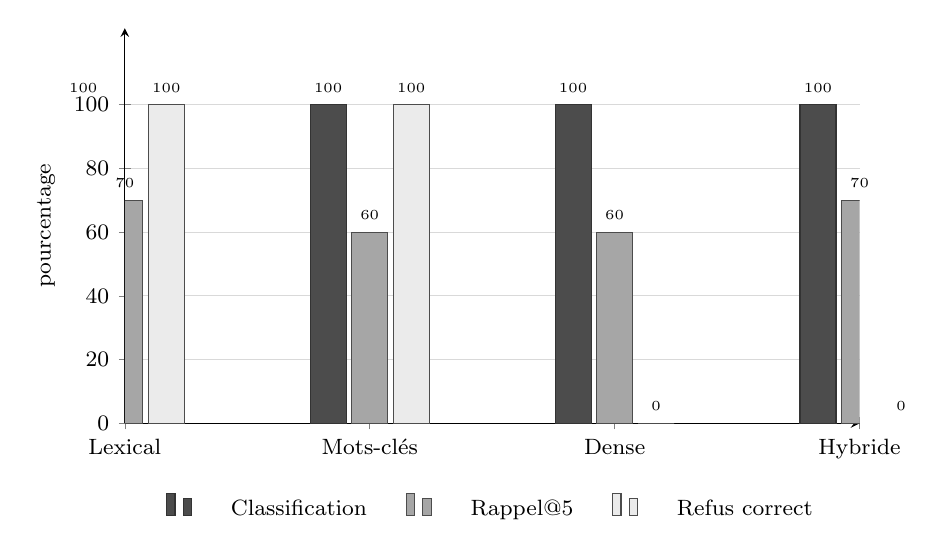
\begin{tikzpicture}
\begin{axis}[
  width=0.9\textwidth, height=6.6cm,
  ybar, bar width=13pt, enlarge x limits=0.20,
  ymin=0, ymax=124, ytick={0,20,40,60,80,100},
  ylabel={\footnotesize pourcentage},
  symbolic x coords={Lexical,Mots-clés,Dense,Hybride},
  xtick=data,
  tick label style={font=\footnotesize},
  label style={font=\footnotesize},
  legend style={font=\footnotesize,at={(0.5,-0.16)},anchor=north,
                legend columns=3,draw=none,column sep=1.2em},
  ymajorgrids, grid style={black!15},
  nodes near coords,
  every node near coord/.append style={font=\tiny,yshift=1pt,
     /pgf/number format/precision=0,/pgf/number format/fixed},
  axis lines=left]
\addplot[fill=black!70,draw=black!80] coordinates {(Lexical,100)(Mots-clés,100)(Dense,100)(Hybride,100)};
\addplot[fill=black!35,draw=black!70] coordinates {(Lexical,70)(Mots-clés,60)(Dense,60)(Hybride,70)};
\addplot[fill=black!8,draw=black!70]  coordinates {(Lexical,100)(Mots-clés,100)(Dense,0)(Hybride,0)};
\legend{Classification,Rappel@5,Refus correct}
\end{axis}
\end{tikzpicture}
\caption{Performance comparée des quatre moteurs sur les trois indicateurs du protocole}
\label{fig:moteurs}
\source{campagne d'évaluation du 27 août 2026.}
\end{figure}

Le moteur dense perd dix points de rappel sur le moteur lexical --- 60~\% contre 70~\% --- et se situe au niveau du simple témoin par mots-clés. Surtout, il fait tomber le taux de refus correct de 100~\% à 0~\% : les huit questions auxquelles le système doit refuser de répondre reçoivent toutes une réponse.

Le moteur hybride égale le lexical au rappel mais hérite du défaut de refus. Il ne rapporte donc rien et coûte l'intégralité de la garantie.

\subsubsection{L'explication}

Le premier réflexe devant un tel résultat est de suspecter un seuil mal réglé. Une sonde a été écrite pour l'éprouver, sur trois couples témoins dont la proximité attendue était connue d'avance. Elle rend 0,644 pour un couple qui doit être proche, mais 0,505 et 0,538 pour deux couples qui doivent être lointains --- l'un des couples étrangers se plaçant \emph{au-dessus} d'un couple lointain.

L'ordre lui-même est donc faux. Un pouvoir de séparation de 0,106 sur une échelle où toutes les valeurs tiennent entre 0,50 et 0,64 signifie qu'aucune valeur de seuil ne sépare quoi que ce soit. Le défaut ne vient pas du réglage mais de l'adéquation entre le modèle et le corpus : \emph{nomic-embed-text} est massivement anglophone, tandis que les fiches du village font deux ou trois mots de français. L'essai des préfixes de tâche recommandés par le modèle dégrade encore la séparation, de 0,023.

Ce diagnostic explique aussi l'effondrement du refus. Le refus repose sur un seuil de similarité en deçà duquel aucune source n'est retenue. Dans un espace où tout est également proche de tout, aucune requête ne tombe jamais sous le seuil : le système trouve toujours cinq documents et ne refuse jamais rien.

\subsubsection{Ce qui a été retenu}

Le moteur lexical est le seul inscrit dans l'ordre de résolution livré. Le dense et l'hybride demeurent enregistrés au catalogue des moteurs, comme le témoin par mots-clés et pour la même raison : ce sont des instruments de mesure, non des moteurs de repli. Un test automatisé retient la décision et échouerait si l'ordre livré venait à changer sans nouvelle mesure.

\subsubsection{Un incident méthodologique qui vaut d'être rapporté}

Une première campagne de mesure avait donné un rappel@5 de 20~\% pour trois moteurs sur quatre et de 0~\% pour le quatrième. Ces valeurs, identiques quel que soit le moteur, auraient dû alerter dès le matin : un indicateur qui ne bouge jamais, quoi qu'on change, ne mesure pas ce qu'on croit.

Le défaut tenait à la définition de la pertinence. Le rappel comparait les fragments attendus aux seuls \emph{titres} des sources. Or le titre d'une fiche produit est sa référence et sa désignation --- \guillemotleft~BTQ12-0038 --- Collier~\guillemotright{} --- tandis que le corps de métier vit dans l'extrait : \guillemotleft~Collier --- Vannerie --- MINTCHOUGOM SIDONIE~\guillemotright. Un jeu de questions visant les corps de métier ne pouvait donc jamais valider une fiche produit, quelle que soit sa pertinence réelle.

La mesure refaite sur le titre \emph{et} l'extrait donne les valeurs du tableau~\ref{tab:moteurs}, contre 20~\%, 0~\%, 20~\% et 20~\% respectivement avant correction. Il ne s'agit pas d'un assouplissement destiné à obtenir un meilleur chiffre : une source dont l'extrait retrouvé parle de vannerie \emph{est} une source sur la vannerie. C'est la définition de la pertinence qui était fausse, non son seuil.

Cet incident est rapporté plutôt que tu, et les deux séries sont conservées au dépôt. La décision d'écarter la branche dense avait été prise sur la seule colonne du refus, qui était valide ; la mesure corrigée la renforce plutôt qu'elle ne la fragilise, puisqu'elle établit en outre une infériorité de rappel. La conclusion était juste, la preuve ne l'était pas ; elle l'est désormais.

\subsection{Synthèse de la discussion}

\begin{table}[H]
\centering
\caption{Statut des hypothèses au regard des résultats}
\label{tab:hypotheses}
\singlespacing
\begin{tabularx}{\textwidth}{@{}p{1.1cm}p{2.6cm}X@{}}
\toprule
\entete{Réf.} & \entete{Statut} & \entete{Élément probant}\\
\midrule
H1 & \textbf{Confirmée}, au-delà de son énoncé & 21,0 \% des ventes non rattachables au parc, soit 20,2 \% du chiffre d'affaires ; quantité absente sur 100 \% des lignes ; identité du vendeur absente de tout support\\
H2 & \textbf{Confirmée}, avec réserve & Huit indicateurs produits par agrégation ; un écart de caisse de 162 525 F rendu décidable par le journal et l'arrêté ; la ventilation par artisan reste bornée par la qualité de la source\\
H3 & \textbf{Infirmée} & Rappel@5 de 60 \% contre 70 \% pour le lexical ; refus correct effondré de 100 \% à 0 \% ; ordre des similarités erroné à la sonde\\
\bottomrule
\end{tabularx}
\onehalfspacing
\source{élaboré par l'auteur.}
\end{table}

L'hypothèse générale --- qu'un système d'information centralisé enrichi d'intelligence artificielle améliore le suivi des activités et renforce la valorisation --- est confirmée quant au suivi, établi par H1 et H2. Elle l'est aussi quant à la valorisation, mais par un chemin différent de celui qui avait été envisagé : c'est la branche lexicale, et non la branche vectorielle, qui rend l'information accessible en langage naturel. L'apport d'intelligence artificielle demeure, il ne repose simplement pas sur la technique présumée.

\section{Présentation des résultats}
\label{sec:4-2}

\subsection{Description de la solution obtenue}

La solution livrée est une application web modulaire de près de 37~500~lignes réparties sur six modules et trente-quatre tables. Elle couvre la chaîne complète de l'activité du village : de l'attribution d'un espace locatif à un artisan jusqu'au reversement des sommes qui lui reviennent, en passant par le dépôt de ses produits, leur validation, leur vente, l'écriture en caisse et la production des indicateurs.

\subsubsection{Performances du dispositif d'intelligence artificielle}

Dans sa configuration livrée, l'assistant classe correctement les 48~questions du jeu d'évaluation, atteint un rappel@5 de 70~\% --- sept des dix questions descriptives à réponse connue voient la source attendue figurer dans les cinq premières --- et refuse explicitement les huit questions sans réponse au corpus. Sur l'ensemble des campagnes, le contrôle des chiffres n'a laissé passer aucun nombre non fondé.

La justesse de classification à 100~\% mérite un commentaire, car un tel chiffre appelle la suspicion plutôt que la satisfaction. Il s'explique par la nature du routeur : celui-ci ne prédit pas une catégorie, il reconnaît une intention dans un catalogue fermé au moyen d'un score de termes. Sur un jeu de questions formulées dans le vocabulaire du domaine, ce mécanisme ne se trompe pas. Il se tromperait sur une question formulée hors de ce vocabulaire, et le comportement est alors conçu pour être sûr : le doute renvoie vers la branche descriptive, qui ne produira aucun chiffre.

\subsubsection{Un écart entre la règle annoncée et la règle appliquée}

L'analyse de la feuille des commissions a fait apparaître un résultat qui ne relève d'aucune hypothèse et qui mérite d'être rapporté, parce qu'il conditionne la façon dont le système doit représenter la commission.

Le taux annoncé est uniforme et vaut 10~\%. Sur les 95~décharges enregistrées, le taux effectivement retenu s'établit à 9,93~\% sur les lignes commissionnées et à 8,19~\% sur l'ensemble de la feuille. L'écart entre ces deux valeurs tient à deux mécanismes que le document ne sépare pas : cinq décharges à commission nulle portant sur 218~000~francs~CFA de ventes, dont plusieurs portent la mention \guillemotleft~RNF~\guillemotright{} sans qu'aucune règle écrite ne fonde l'exonération ; et deux dépenses --- 5~000~francs~CFA d'emballage, 2~000~francs~CFA de frais postaux --- imputées en commission négative alors qu'il s'agit de sorties de caisse.

Ce constat a orienté deux décisions de conception. D'abord, le taux de commission est historisé par date d'effet et figé sur chaque vente à son enregistrement : le taux appliqué reste ainsi lisible même s'il change ensuite. Ensuite, une dépense ne peut structurellement pas s'imputer sur une commission, puisqu'elle constitue un mouvement de caisse enregistré comme tel dans le brouillard. La colonne de recette de commission redevient de ce fait lisible pour ce qu'elle est.

L'exonération, en revanche, n'est pas représentée : le système applique le taux en vigueur sans exception. C'est un choix assumé, faute d'une règle écrite à implémenter. Le formaliser --- qui peut exonérer, sur quel motif, avec quelle trace --- est une question qui relève de la coordination et non du développement.

\subsubsection{Points forts}

Le premier point fort est la \textbf{garantie sur les montants}. L'architecture rend structurellement impossible qu'un chiffre soit produit par proximité textuelle. Cette garantie ne repose pas sur une consigne donnée au modèle de langage, qui pourrait être contournée, mais sur le fait que le modèle n'a accès à aucune source d'où un montant pourrait venir. Elle est en outre doublée d'un contrôle mécanique, qui a laissé passer zéro chiffre sans source sur l'ensemble des campagnes.

Le deuxième est le \textbf{fonctionnement sans connexion}. Le module de gestion ne dépend d'aucun service externe. L'assistant lui-même fonctionne hors ligne dans sa configuration livrée, puisque la branche lexicale ne suppose aucune vectorisation externe et que le repli de rédaction est le comportement nominal d'origine.

Le troisième est la \textbf{traçabilité}. Toute création, modification ou action sensible est journalisée avec l'identité de son auteur, et le journal de caisse est immuable : une correction procède d'une écriture inverse, jamais d'une modification. Le brouillard montre ainsi à la fois le chiffre juste et le fait qu'il a été faux.

Le quatrième est le \textbf{coût de mise en service nul} pour le cœur du système, qui répond directement au précédent d'un projet antérieur abandonné pour ce motif.

\subsubsection{Limites}
\label{sec:4-2-3}

Cinq limites doivent être énoncées, et leur énoncé conditionne la crédibilité de ce qui précède.

La \textbf{première} est que les prix ne représentent pas les conditionnements. Un produit vendu en plusieurs formats à des prix distincts se modélise par autant de produits séparés. Le système contient le défaut par un signalement explicite plutôt qu'il ne le corrige, comme exposé au chapitre~3.

La \textbf{deuxième} est que l'autorisation repose entièrement sur le contrôle porté par chaque action, sans couche de politique d'accès déclarée au niveau des modèles. Ce choix est assumé sous contrainte de délai et gardé par un test de conventions qui parcourt tous les écrans ; il devra être repris si le système s'ouvre à d'autres profils.

La \textbf{troisième} est que l'alerte de rupture de stock n'atteint que deux de ses trois destinataires. Les sections Production et Commercialisation la reçoivent ; l'artisan ne la reçoit pas, faute de disposer d'un compte dans le système. Le message porte en compensation le nom de l'artisan et le numéro de son espace, de sorte que la section sait qui appeler.

La \textbf{quatrième} est que l'espace artisan reste au stade de la maquette. Sa réalisation complète suppose un compte par artisan, qui conditionne aussi la levée de la limite précédente.

La \textbf{cinquième} est que le rappel@5 de 70~\% laisse trois questions sur dix sans source pertinente dans les cinq premiers résultats. Ce niveau est acceptable pour un usage d'aide à la recherche, où l'utilisateur voit les sources et juge ; il ne le serait pas pour un usage automatisé sans supervision, qui n'est pas celui du système.

\subsection{Interfaces principales de l'application}

Les écrans suivants constituent les points d'entrée du système. Les captures correspondantes sont à insérer à l'emplacement indiqué.

\capture{Tableau de bord du pilotage}{Indicateurs clés : chiffre d'affaires de la période, recettes de commission, soldes de caisse, dettes envers les artisans, ventes ventilées par axe et alertes de stock.}

\capture{Écran de vente et brouillard de caisse}{À gauche, la sélection préalable d'une boutique puis le choix des produits de cette seule boutique, avec calcul de la commission et figement des valeurs. À droite, le journal chronologique des mouvements, numérotés par section, avec le solde après chaque écriture.}

\capture{Assistant d'interrogation en langage naturel}{Question posée en français, réponse produite et sources affichées sous la réponse. La capture doit montrer une question d'agrégation et une question descriptive, afin de rendre visibles les deux branches.}

\capture{Portail public --- accueil et catalogue}{Vitrine présentant le village, les artisans mis en avant et le catalogue des produits validés et publiés, sans fonction de commande ni de paiement.}

\section{Coût estimatif du projet}
\label{sec:4-3}

Le projet a été conduit avec les moyens matériels disponibles et le travail fourni dans le cadre d'un stage académique. Le tableau~\ref{tab:cout} valorise l'ensemble au prix du marché local, afin que la structure dispose d'un ordre de grandeur en cas de reprise, d'extension ou de transposition à un autre village artisanal.

\begin{table}[H]
\centering
\caption{Coût estimatif du projet}
\label{tab:cout}
\singlespacing
\begin{tabularx}{\textwidth}{@{}Xrrr@{}}
\toprule
\entete{Poste} & \entete{Qté} & \entete{P.U. (FCFA)} & \entete{Total (FCFA)}\\
\midrule
\multicolumn{4}{@{}l}{\emph{Développement}}\\
Analyse de l'existant et collecte de terrain & 4 j & 25 000 & 100 000\\
Conception et modélisation & 3 j & 25 000 & 75 000\\
Développement des modules de gestion & 16 j & 25 000 & 400 000\\
Reprise et qualification des données & 2 j & 25 000 & 50 000\\
Volet intelligence artificielle & 4 j & 25 000 & 100 000\\
Portail public & 3 j & 25 000 & 75 000\\
Tests, documentation et manuel utilisateur & 4 j & 25 000 & 100 000\\
\midrule
\multicolumn{4}{@{}l}{\emph{Infrastructures}}\\
Poste de développement et de déploiement & 1 & 450 000 & 450 000\\
Connexion Internet, durée du projet & 3 mois & 15 000 & 45 000\\
Serveur local, base de données, cadriciel & --- & 0 & 0\\
Nom de domaine et hébergement du portail, 1\textsuperscript{re} année & 1 & 72 000 & 72 000\\
\midrule
Provision pour imprévus (10 \%) & --- & --- & 146 700\\
\midrule
\textbf{Coût total valorisé} & & & \textbf{1 613 700}\\
\emph{dont dépense annuelle récurrente} & & & \emph{72 000}\\
\bottomrule
\end{tabularx}
\onehalfspacing
\source{élaboré par l'auteur, prix du marché local à la date de rédaction.}
\end{table}

La ligne la plus importante de ce tableau est celle des coûts nuls. Le choix d'un cadriciel libre, d'un système de gestion de base de données libre et d'un déploiement en réseau local ramène à zéro la dépense récurrente du cœur du système. Seule la mise en ligne du portail public engage une dépense annuelle de 72~000~francs~CFA, isolée ici pour que la coordination puisse en décider séparément.

Ce coût est valorisé et non décaissé. Rapporté au reste à recouvrer de l'exercice~2026, soit 1~959~000~francs~CFA, il représente 82~\% d'une seule année de redevances non perçues. La comparaison ne prétend pas établir un retour sur investissement --- le système ne recouvre pas les redevances, il les rend visibles --- mais elle situe l'ordre de grandeur de l'enjeu.

\section{Rétrospective du projet}
\label{sec:4-4}

\subsection{État actuel}

À la date de rédaction, les six modules sont réalisés et la chaîne complète --- attribution, dépôt, vente, écriture en caisse, compte artisan, campagne de reversement --- fonctionne sur les données réelles du village. Le tableau de bord est en service, l'assistant d'interrogation est opérationnel et mesuré, et le portail public est complet en local. Une suite de tests automatisés couvre les règles de gestion, les habilitations et les conventions d'écriture, et la base est reconstructible en une commande à partir des jeux d'amorçage. Trois éléments restent au stade de la maquette ou de la perspective : l'espace artisan, le canal de notification par courriel et l'échéancier automatisé des redevances, ce dernier ayant été explicitement retiré du périmètre.

\subsection{Apports du projet}

\subsubsection{Sur le plan académique}

Le projet a permis de conduire un cycle complet de traitement de données, de la source manuscrite jusqu'à l'indicateur et à l'évaluation d'un dispositif d'intelligence artificielle. Il a surtout imposé une leçon que les travaux dirigés transmettent mal : la constitution du gisement de données représente la part majeure de l'effort, et la qualité des données conditionne tout ce qui vient après. Il a également donné l'occasion de produire, de mesurer et d'écarter une technique sur des bases chiffrées --- un résultat négatif documenté se démontre, là où une fonctionnalité seulement affirmée ne se défend pas.

\subsubsection{Sur les plans professionnel et personnel}

Le travail a été conduit en interaction avec une structure réelle, dont les besoins ne sont pas exprimés en termes informatiques et dont les données ne se présentent pas sous forme exploitable. Il a fallu observer des processus, interroger des agents, arbitrer des règles de gestion avec la coordination et distinguer ce qui relève d'un choix technique de ce qui relève d'une décision de la structure.

L'expérience la plus formatrice a porté sur les contraintes non techniques. Le facteur déterminant du projet n'a pas été la difficulté d'implémentation mais le budget de déploiement, dont un précédent avait déjà démontré le caractère bloquant ; c'est lui qui a commandé les choix technologiques. Le projet ayant été mené seul et sous contrainte de délai stricte, il a enfin imposé de traiter le manque de relecture par des dispositifs mécaniques plutôt que par l'attention, et de consigner chaque décision au moment où elle est prise.

\subsection{Difficultés rencontrées}

La difficulté la plus coûteuse n'a pas été technique. À trois reprises, une règle a été inventée par déduction plutôt qu'établie sur les données : un tarif de redevance au mètre carré, cohérent sur le papier et qui n'a jamais produit un seul montant ; l'affirmation que le sous-sol ne comportait aucun espace locatif, démentie par un relevé qui y nomme la redevance la plus élevée du parc ; et la supériorité présumée des plongements denses. Le fil est identique dans les trois cas : \textbf{une règle inventée par déduction ne se fait jamais démentir tant que rien ne la remplit}. La troisième est tombée en quatre minutes, pour un motif qui distingue les trois cas --- on avait cette fois écrit la sonde capable de la démentir. Les deux échecs précédents n'ont pas manqué de raisonnement, ils ont manqué d'un objet capable de dire non.

Une deuxième famille de difficultés tient aux dispositifs de vérification qui semblent vérifier et mesurent autre chose. L'instrument d'évaluation était aveugle aux moteurs nouvellement ajoutés ; un indicateur mesurait une propriété des titres plutôt que la pertinence des sources ; un événement métier était correctement émis et écouté par personne, sans qu'aucun test ne puisse le révéler puisqu'ils vérifiaient l'émission et non l'arrivée. La règle qui en découle est qu'une règle de gestion n'est tenue que lorsqu'un test décrit son \emph{effet observable}, et non l'existence du mécanisme censé la produire.

Une troisième famille tient aux pannes que le repli absorbe. Un identifiant de modèle retiré du service ne dégrade pas la réponse : il la refuse, et le repli le fait en silence. Un échec de vérification de certificat produit le même effet. Dans les deux cas, le système paraissait fonctionner. La règle retenue est qu'\textbf{un repli doit être silencieux pour l'utilisateur et bavard pour le développeur} : un système dégradé qui se tait des deux côtés est indiscernable d'un système qui fonctionne.

Une dernière difficulté tient aux zones que les données ne permettent pas de combler : des ventes rattachées à aucun espace, des locaux absents du relevé de recouvrement, des exonérations de commission sans règle écrite. Ces points ont été adressés à la coordination sous forme de questions écrites, et l'hypothèse retenue à défaut de réponse est consignée pour chacun. Une question restée sans réponse, signalée comme telle avec l'hypothèse qui en tient lieu, est plus solide qu'un silence comblé par une invention.

\vspace{1em}
\noindent\textbf{Conclusion partielle.} Ce chapitre a confronté les trois hypothèses aux mesures produites : deux sont confirmées, la troisième est infirmée par un protocole explicite dont les fichiers de résultats sont versionnés. Il a présenté la solution livrée, ses quatre points forts et ses cinq limites, puis le coût valorisé du projet, dont la structure fait apparaître un coût récurrent nul pour le cœur du système. Il a enfin dressé la rétrospective du travail, dont les difficultés les plus coûteuses ne furent pas d'implémentation mais de méthode : des règles déduites sans être éprouvées, des instruments de vérification qui mesuraient autre chose, et des défaillances que le repli rendait invisibles.
